\chapter{Cơ sở lý thuyết}
\label{chapter2}
Chương này em sẽ trình bày những kiến thức cần có để xây dựng được một mạng hình sao sử dụng công nghệ truyền thông LoRa. Đây là những kiến thức cơ bản về LoRa, đa truy nhập trong mạng không dây, các thiết bị phần cứng được sử dụng cũng như một số công cụ phần mềm hỗ trợ thiết kế và lập trình.
\section{Công nghệ LoRa}  
$LoRa^{TM}$ (Long Range Radio) \cite{2} là một công nghệ truyền thông không dây có phạm vi hoạt động lớn, tiêu tốn ít năng lượng và sử dụng dải tần miễn phí (unlicensed radio spectrum), dải tần này được sử dụng trong công nghiệp, khoa học và y tế (ISM band). LoRa được phát triển bởi Cycleo SAS (sau này được mua lại bởi SemTech). Mục đích tạo ra công nghệ LoRa là nhằm loại bỏ repeater, giảm chi phí đầu tư vào thiết bị, tăng cường thời gian hoạt động, tăng dung lượng mạng và hỗ trợ cho mạng có số thiết bị lớn. Công nghệ LoRa nằm lớp vật lý, được sử dụng cho truyền thông phạm vi lớn. Hầu hết công nghệ không dây sử dụng kỹ thuật điều chế số theo tần số tín hiệu FSK (Frequency Shift Key). Tuy nhiên, LoRa lại sử dụng kỹ thuật điều chế Chirp Spread Spectrum (CSS) để tiết kiệm năng lượng nhằm tăng khoảng cách truyền. LoRa là công nghệ đầu tiên sử dụng kỹ thuật điều chế CSS được thương mai hóa. Trước đó, kỹ thuật điều chế CSS chỉ được dùng trong quân sự và hàng không vũ trụ. Nhờ những ưu điểm về năng lượng và tầm hoạt động, LoRa phù hợp để ứng dụng trong mạng WSN cũng như các thiết bị IoT.
\subsection{Kỹ thuật điều chế CSS}
Theo tài liệu \cite{3}, LoRa dựa trên kỹ thuật điều chế Chirp Spread Spectrum (CSS) (Hình \ref{refhinh2_1}{}). CSS được xem là một kỹ thuật Direct-Sequence Spread Spectrum. CSS phù hợp với nhu cầu mạng IoT bởi vì nó cho phép chống nhiễu tốt, phạm vi sử dụng lớn và tiêu thụ ít năng lượng. Trong kỹ thuật trải phổ CSS, tín hiệu chirp được mô tả bằng hàm pha tức thời $\phi(t)$ hoặc một hàm thời gian đặc biệt $f_c(t)$. $f_c(t)$ được gọi là hàm tín hiệu chirp chưa được xử lý (the raw chirp) do:
\begin{itemize}
\item Khi tăng tuyến tính, một tín hiệu up-chirp bắt đầu từ $-\dfrac{B}{2}$ đến $\dfrac{B}{2}$,
\item Khi giảm tuyến tính, một tín hiệu down-chirp bắt đầu từ $\dfrac{B}{2}$ đến $-\dfrac{B}{2}$, 
\end{itemize}
trong đó, B là băng thông của d ải tần ISM được sử dụng. Hàm $f_c(t)$ được xác định bởi công thức:
\begin{equation}
f_c(t) = \pm \dfrac{B}{T_s}t
\end{equation}
trong đó $T_s$ là chu kỳ ký hiệu (symbol period). Mối quan hệ giữa băng thông và chu kỳ ký hiệu được thể hiện trong công thức $T_s = \dfrac{2^{SF}}{B}$ trong đó SF là hệ số trải phổ nằm trong khoảng [7,..., 12]. $D_s$ là tỷ lệ ký hiệu trong tín hiệu được truyền và $D_b$ là tỷ lệ bit, $D_s =\dfrac{D_b}{SF}$.
\par 
Trong LoRa, một ký hiệu được tạo từ SF bit nhị phân. Mỗi ký hiệu được mô tả bởi một chirp duy nhất. Các chirp khác nhau trực giao với nhau để khi được khôi phục ở bên nhận các ký hiệu tránh được nhiễu (Inter-symbol interference). Nếu chúng ta có bộ M ký hiệu, ký hiệu m, $m \in [0, M-1]$, thu được bởi chễ raw chirp $f_c(t)$ và $\tau_m = \dfrac{m}{B}$. Những chirp nằm bên ngoài khoảng $[-\dfrac{T_s}{2}, \dfrac{T_s}{2}]$ được chuyển dịch chu kỳ $[-\dfrac{T_s}{2}, -\dfrac{T_s}{2} + \tau_m]$. Do đó, chirp liên quan đến việc truyền ký tự thứ m được chia làm hai phần:
\begin{itemize}
\item Nếu  $t \in [-\dfrac{T_s}{2}, -\dfrac{T_s}{2} + \tau_m]$, raw chirp nhỏ hơn $(T_s - \tau_m)$,
\item Nếu $t \in [-\dfrac{T_s}{2} + \tau_m, \dfrac{T_s}{2}]$, raw chirp lớn hơn $\tau_m$.
\end{itemize}
\begin{center}
    \begin{figure}[h]
    \begin{center}
     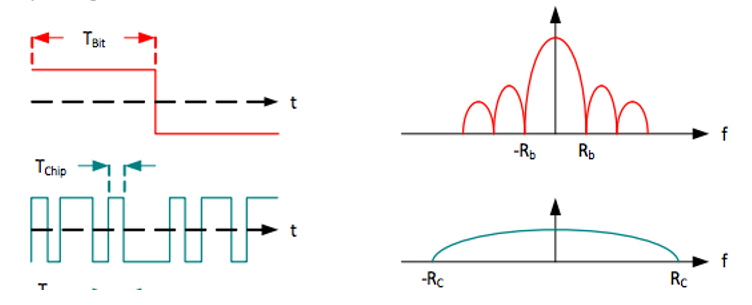
\includegraphics[scale=0.5]{image/hinh2_1}
    \end{center}
    \caption{Nguyên lý điều chế dữ liệu của công nghệ LoRa}
    \label{refhinh2_1}
    \end{figure}
\end{center}
\par
Nhờ sử dụng tín hiệu chirp  mà các tín hiệu LoRa với các tỷ lệ chirp khác nhau có thể hoạt động trong cùng 1 khu vực mà không gây nhiễu cho nhau. Điều này cho phép nhiều thiết bị LoRa có thể trao đổi dữ liệu trên nhiều kênh đồng thời (mỗi kênh cho 1 chirprate).
\subsection{Kiến trúc mạng LoRa}
Một mạng sử dụng công nghệ truyền thông LoRa \cite{4} sẽ được triển khai theo cấu trúc hình sao và gồm hai phần là back-end và front-end (Hình \ref{refhinh2_2}). Phần back-end là máy chủ mạng chứa thông tin nhận được từ các cảm biến. Còn phần front-end chứa module Gateway và các nút (end-device nodes). Gateway có nhiệm vụ làm cầu nối giữa các nút và máy chủ. Thông tin mà Gateway nhận được sẽ được gửi đến máy chủ qua kết nối IP.
\begin{center}
    \begin{figure}[h]
    \begin{center}
     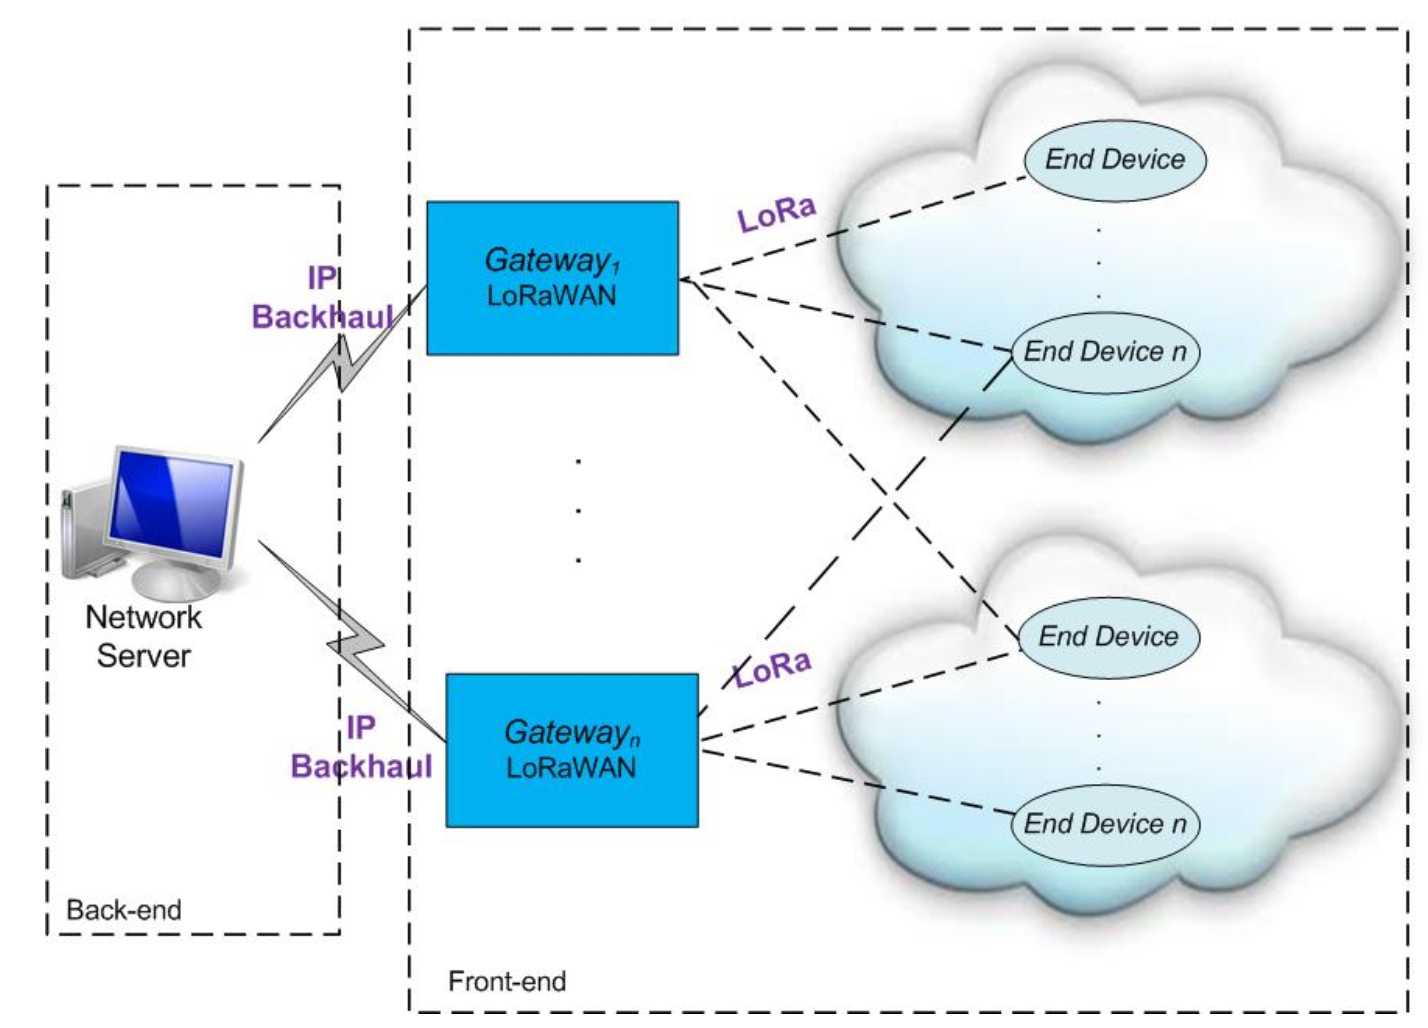
\includegraphics[scale=0.22]{image/hinh2_2}
    \end{center}
    \caption{Kiến trúc mạng LoRa \cite{4}}
    \label{refhinh2_2}
    \end{figure}
\end{center}
\par 
LoRa hoạt động dải tần ISM \cite{4}, tuy nhiên ở mỗi nước (khu vực) thì dải tần này lại khác nhau. Cụ thể là:
\begin{itemize}
\item	Ở Châu Âu, dải tần ISM là: 433MHz hoặc 863-870MHz, gồm có 3 kênh (tương ứng với mỗi dải tần): 433.175 MHz, 433.375 MHz, 433.575 MHz hoặc 868.10 MHz, 868.30 MHz, 868.50 MHz,
\item	Dải tần ISM ở Mỹ là: 902-928MHz,
\item 	Dải tần ISM ở Trung Quốc là: 779-787MHz,
\item 	Ở Úc, dải tần ISM là: 915-928MHz.
\end{itemize}
\par 
Dựa vào cơ chế truyền thông, các nút LoRa (end-device) được chia thành 3 loại \cite{4} gồm:
\begin{itemize}
\item	Class A (Baseline): Khung truyền được chia thành uplink và downlink, bao gồm 1 khe thời gian uplink, tiếp theo là 2 khe thời gian downlink. Thiết bị loại này chỉ có thể nhận dữ liệu từ máy chủ sau khi nó đã gửi dữ liệu,
\item Class B (Beacon): Thiết bị đầu cuối mở thêm một khe nhận trong khoảng thời gian downlink, cùng thêm hai khe thời gian được chỉ định trong loại A. Ngoài khả năng nhận dữ liệu như các thiết bị loại A, các thiết bị loại B cũng có thể sử dụng một loạt khe nhận được kích hoạt bởi các bản tin kiểu Beacon đươc gửi từ gateway,
\item	Class C (Continuous): Các thiết bị loại này có thể nhận dữ liệu bất kể khi nào trừ lúc truyền dữ liệu.
\end{itemize}
    \begin{figure}[h]
    \begin{center}
     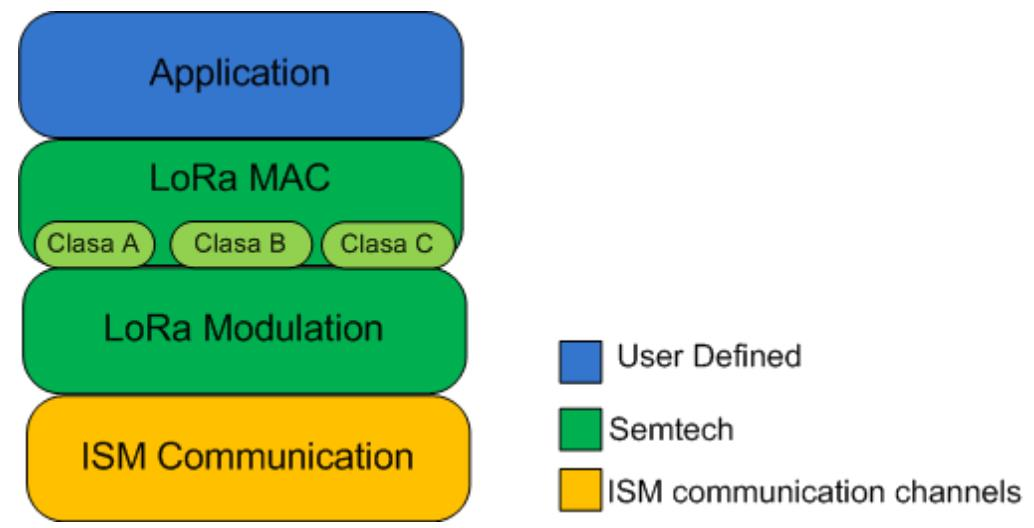
\includegraphics[scale=0.43]{image/hinh2_3}
    \end{center}
    \caption{Kiến trúc các lớp của thiết bị LoRa \cite{4}}
    \label{refhinh2_3}
    \end{figure}
Thiết bị loại A là đơn giản nhất và đảm bảo tiêu thụ năng lượng tối thiểu nhưng lại bị hạn chế khả năng nhận tin nhắn. Nên theo tiêu chuẩn LoRa, các thiết bị phải thực hiện tối thiểu được cơ chế truyền thông loại A. Hình \ref{refhinh2_3} sẽ cho ta thấy rõ hơn cấu trúc các lớp của một thiết bị LoRa.
\subsection{Thông số hoạt động chính của LoRa}
Đối với chipset SX1278 của Semtech, hệ số trải phổ SF (Spreading Factor) có giá trị từ 7 đến 12 \cite{5}. Hệ số SF thể hiện mối quan hệ giữa tốc độ truyền dữ liệu và khoảng cách truyền. Lựa chọn hệ số SF cao có thể làm tăng phạm vi hoạt động nhưng giảm tốc độ truyền dữ liệu và ngược lại. Mỗi ký hiệu được mã hóa bởi một mã có độ dài $2^{SF}$ chip. Do việc mã hóa một ký hiệu bằng nhiều tín hiệu chip, điều này làm ảnh hưởng đến tốc độ truyền dữ liệu. Mỗi quan hệ giữa tốc độ truyền dữ liệu và hệ số SF được thể hiện trong Hình \ref{refhinh2_4}{}a tại các băng thông khác nhau.\\
\begin{figure}[h]
\centering
\subfigure[Tốc độ truyền dữ liệu tương ứng với mỗi hệ số SF.]
  {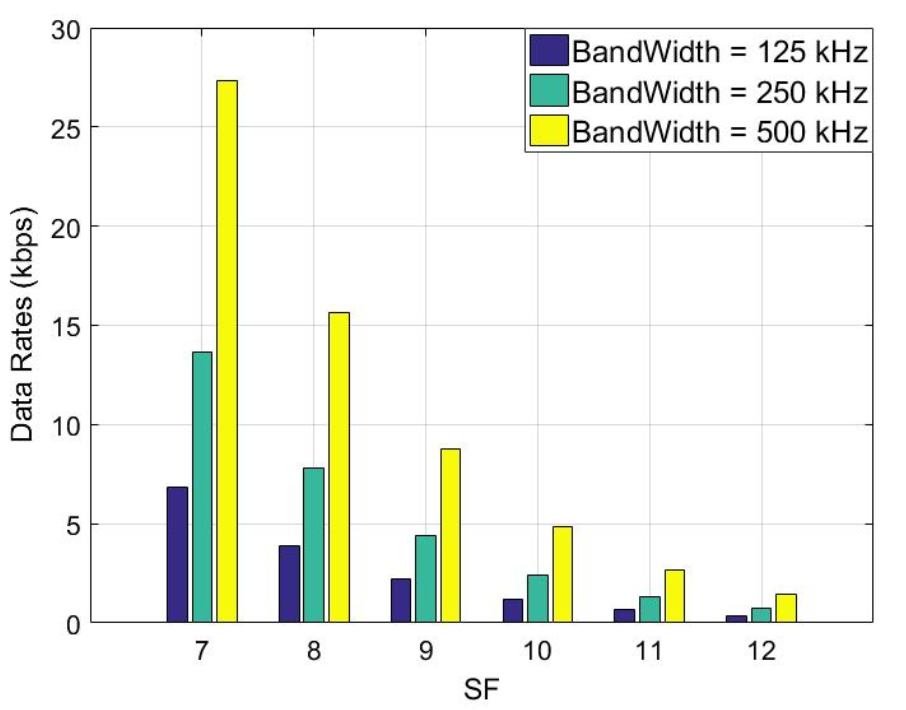
\includegraphics[width=.49\linewidth]{image/hinh2_4}}\hfill
\subfigure[Tốc độ truyền dữ liệu tương ứng với mỗi tốc độ CR.]
  {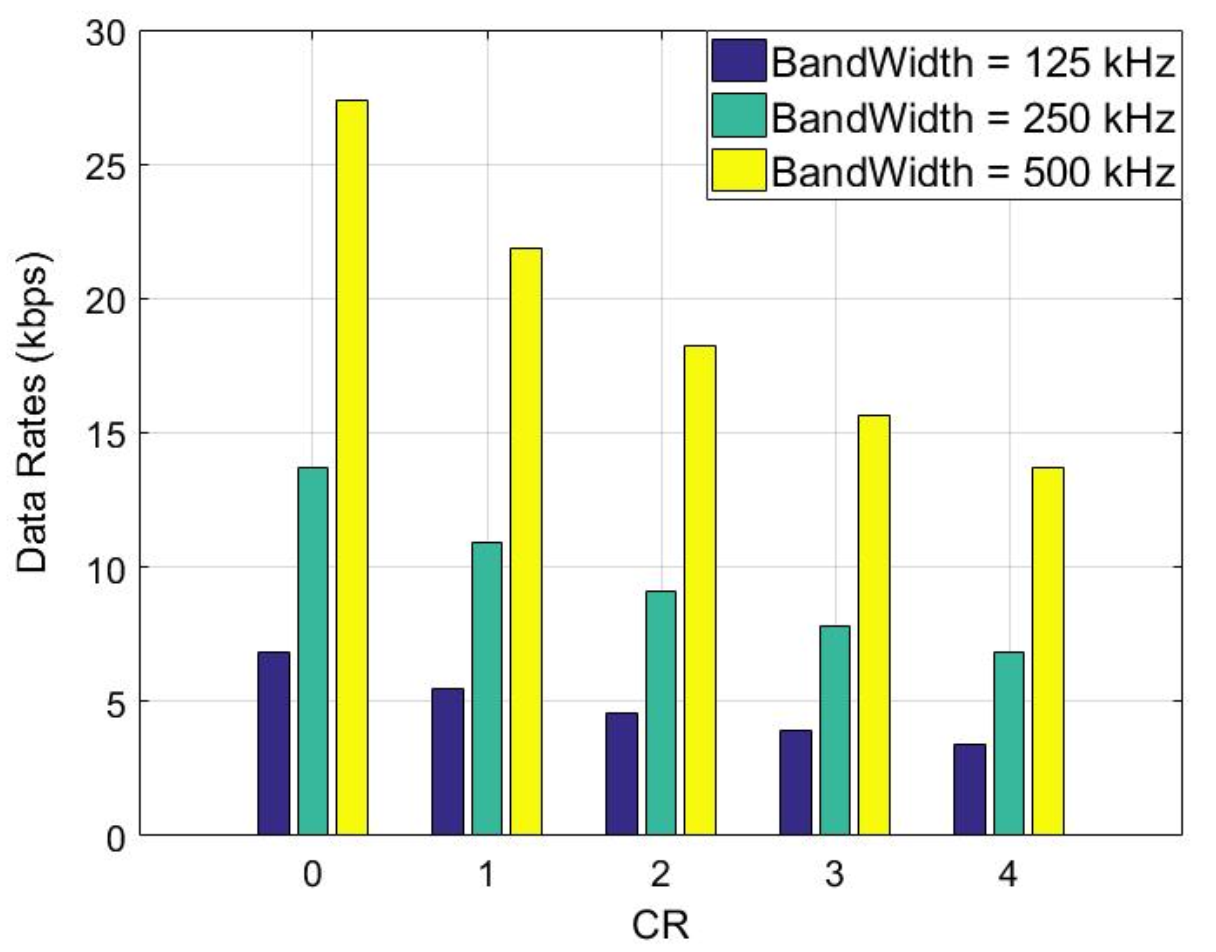
\includegraphics[width=.49\linewidth]{image/hinh2_5}}
\caption{Mối quan hệ giữa tốc độ truyền dữ liệu với các hệ số SF, CR \cite{5}}
\label{refhinh2_4}
\end{figure}
\par 
Theo tài liệu \cite{5}, LoRa thường sử dụng băng thông BW  Bandwidth) có giá trị là 125 KHz nhưng cũng có thể mở rộng lên thành 250 KHz và 500 KHz để truyền tín hiệu. Với băng thông có độ rộng lớn, LoRa hạn chế được nhiễu kênh truyền, hiệu ứng doppler và fading. Máy phát gửi dữ liệu với tốc độ chip bằng với băng thông nên với băng thông là 125 kHz thì tốc độ chip là 125 kcps.
\par 
Tốc độ mã hóa CR (Coding Rate) của chipset SX1278 của SemTech thì CR có 4 giá trị là 4/5, 4/6, 4/7 và 4/8. Nếu tốc độ mã hóa là k/n, thì k là số bit có ích (chứa thông tin được mã hóa) và n là số bit ở đầu ra. Do đó n - k là số bit dự phòng, những bit này cho phép người nhận phát hiện và sửa lỗi trong bản tin nhưng nó cũng làm giảm tốc độ truyền dữ liệu. Tốc độ truyền dữ liệu tương ứng với mỗi CR được thể hiện trong Hình \ref{refhinh2_4}{}b ở mỗi băng thông khác nhau. Ngoài ra, tốc độ truyền dữ liệu cũng phụ thuộc vào độ dài gói tin (Hình \ref{refhinh2_6}). \\
\begin{figure}[h]
\centering
\subfigure[Thời gian truyền gói tin với BW = 125 kHz and CR = 0.]
  {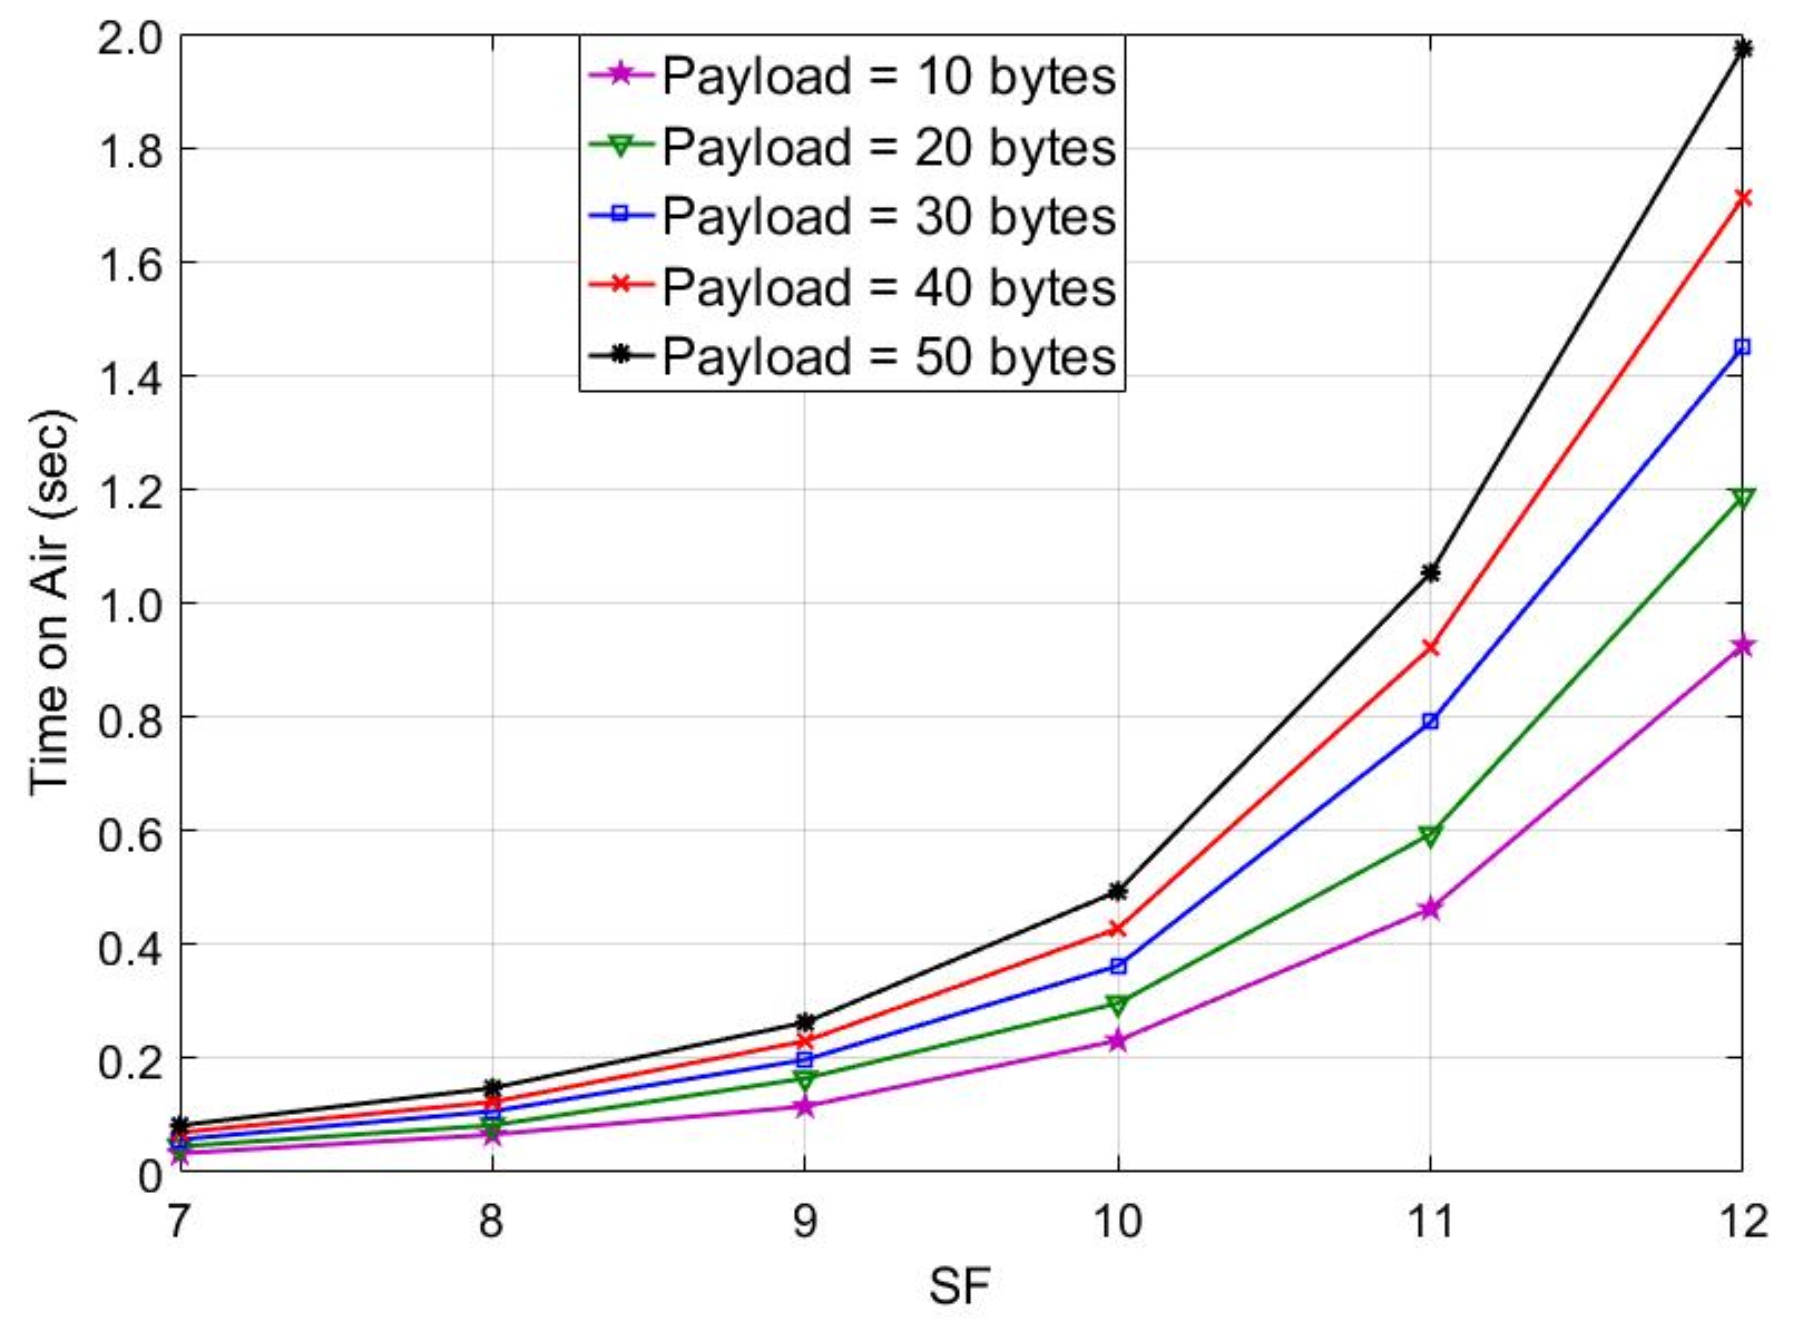
\includegraphics[width=.49\linewidth]{image/hinh2_7a}}\hfill
\subfigure[Thời gian truyền gói tin với BW = 125 kHz and CR = 02.]
  {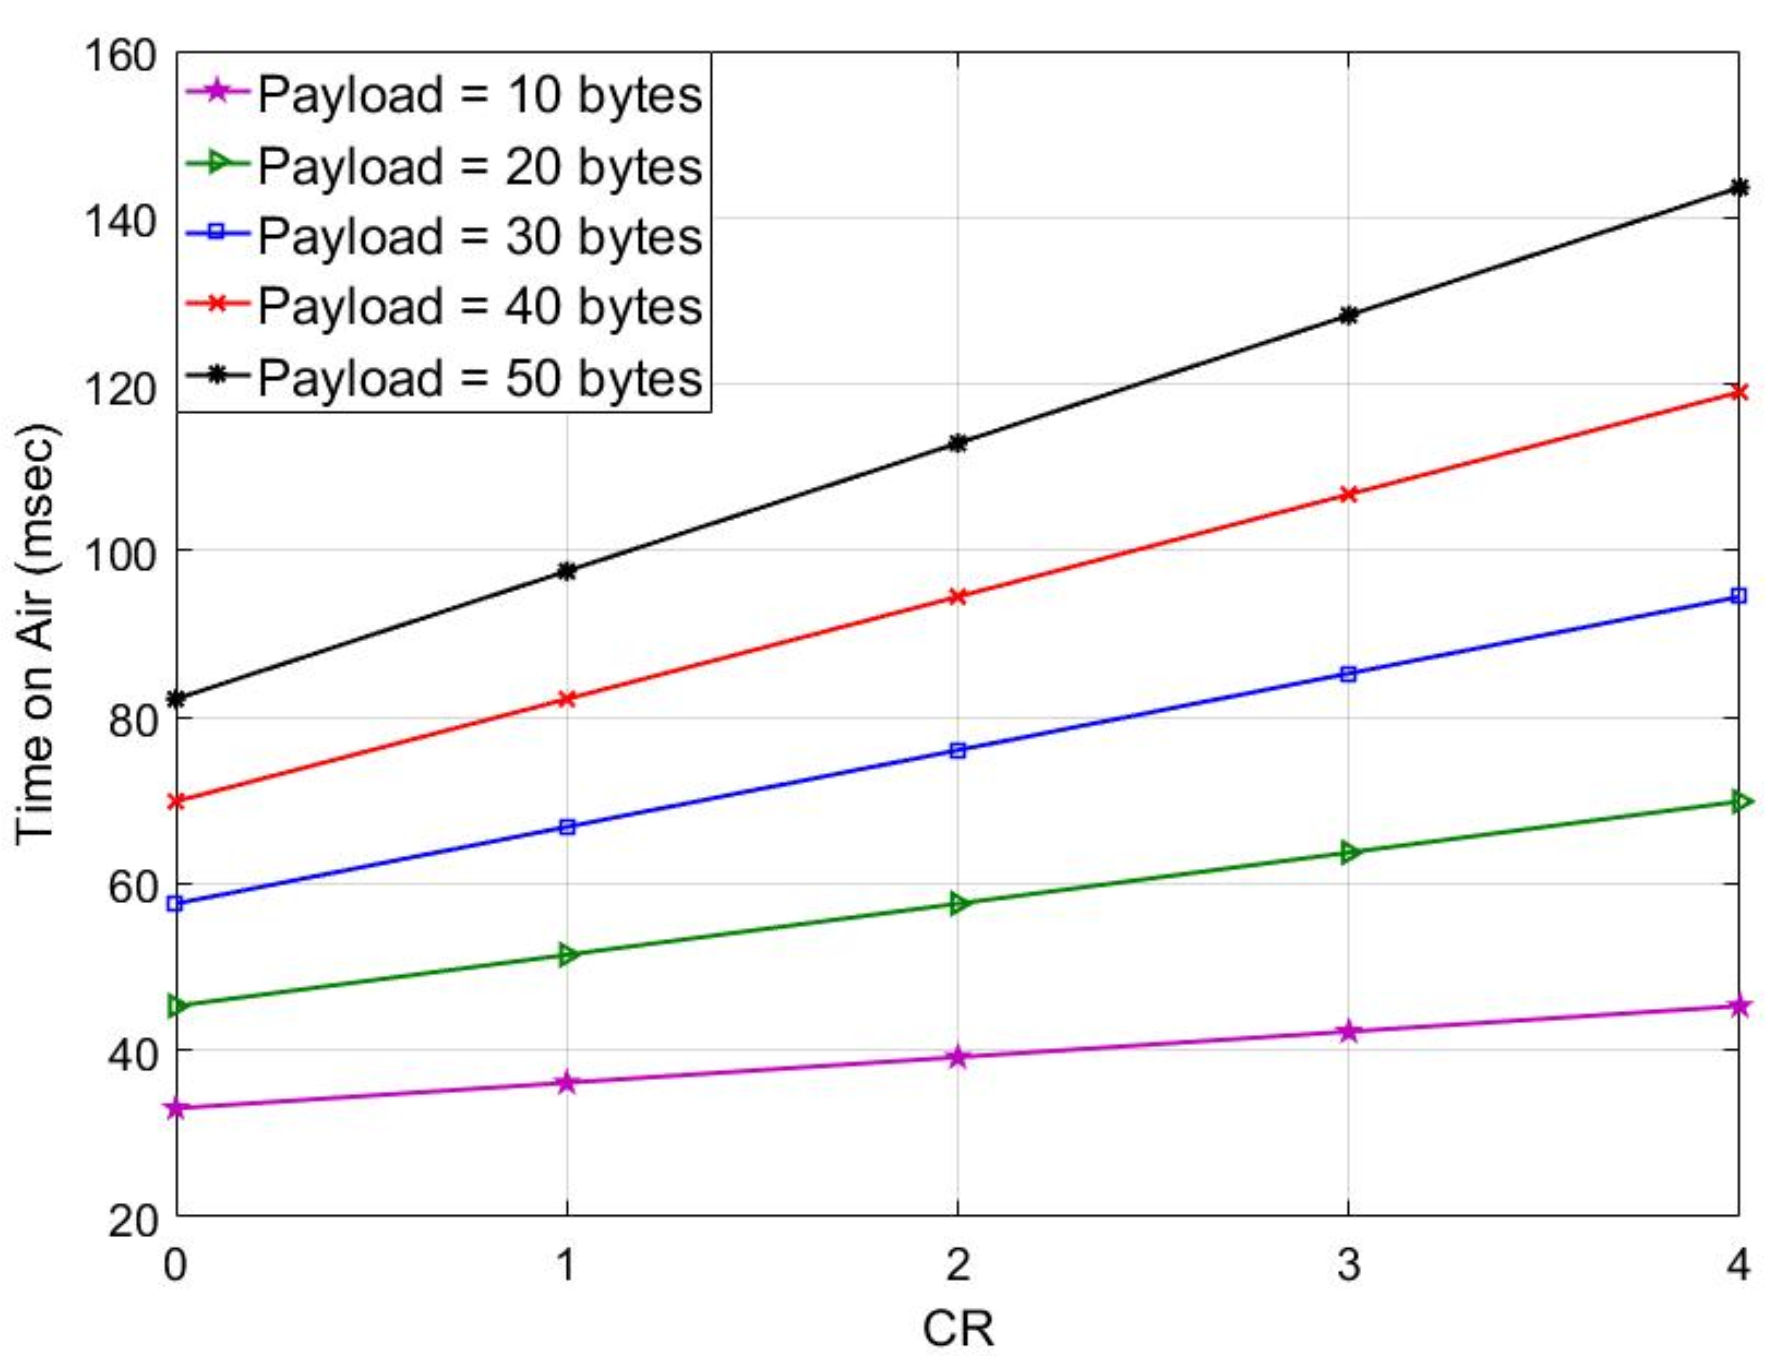
\includegraphics[width=.49\linewidth]{image/hinh2_7b}}
\caption{Thời gian truyền gói tin trong không khí của LoRa. \cite{5}}
\label{refhinh2_6}
\end{figure} 
\begin{center}
    \begin{figure}[h]
    \begin{center}
     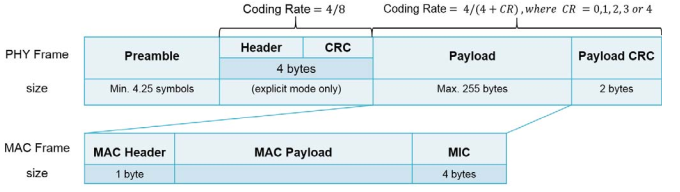
\includegraphics[scale=0.6]{image/hinh2_6}
    \end{center}
    \caption{Cấu trúc một gói dữ liệu được truyền đi \cite{5}.}
    \label{refhinh2_5}
    \end{figure}
\end{center}
\par
Kích thước lớn nhất của một gói tin LoRa là 256 byte, cấu trúc một gói tin (Hình \ref{refhinh2_5}{}) gồm các thành phần sau:
\begin{itemize}
\item  Preamble: là trường chuỗi bit để dò tìm tín hiệu của LoRa trong không gian,\newline
\item  Header: chứa thông tin về kích thước của Playload và xem có Payload CRC hay không. Giá trị của Header cũng được check CRC kèm theo,
\item  Payload: chứa dữ liệu ứng dụng truyền qua LoRa, có kích thước từ 2 đến 255 byte. Trường này còn chứa các trường sau:
	\begin{itemize}
	\item	MAC header: phụ thuộc vào kiểu của frame (là dữ liệu hoặc ACK), phiên bản của giao thức và hướng của nó (uplink hoặc downlink).
	\item	MAC payload: chứa dữ liệu.
	\item 	MIC: được sử dụng như là chữ ký số của dữ liệu.
	\end{itemize}
\item	CRC: là trường tùy chọn và chứa các byte kiểm tra vòng CRC (Cyclic Redundancy Check).
\end{itemize}
\section{Đa truy nhập trong mạng không dây}
Đa truy nhập (Multiple Access) là một kỹ thuật cho phép nhiều thiết bị sử dụng chung một kênh truyền. Kỹ thuật này nằm ở lớp MAC (Medium Access Control), đây là một lớp đặc biệt quan trọng trong những mạng LAN (Local Area Network), trong đó có mạng không dây bởi vì các thiết bị trong mạng này sử dụng chung môi trường truyền.
\par
Giả sử có nhiều thiết bị đang sử dụng kênh truyền, trong cùng một khoảng thời gian với cùng tần số, khi đó sẽ xảy ra hiện tượng va chạm. Do đó, cần phải có một biện pháp kiểm soát các thiết bị tham gia kênh truyền. Ví dụ như một mạng có băng thông là B, có N thiết bị đang tham gia kênh truyền, mạng sử dụng phương pháp ghép kênh phân chia theo tần số FDM (Frequency Division Multiplexing), khi đó băng thông được chia thành N dải tần, mỗi thiết bị sẽ sử dụng một dải tần. Tuy nhiên, với số lượng thiết bị lớn, thì những dải tần này bị chia quá nhỏ, do đó dễ gây nên can nhiễu. Do đó, cần có thêm những phương pháp kiểm soát kênh truyền. Đây là 4 phương pháp điều khiển truy nhập kênh truyền:
\begin{itemize}
\item Đa truy nhập phân chia theo tần số FDMA (Frequency Division Multiple Access): dải tần số sẽ được chia thành các dải tần số nhỏ không chồng lên nhau, và mỗi dải đó được sử dụng bởi một thiết bị khác nhau, 
\item Đa truy nhập phân chia theo thời gian TDMA (Time Division Multiple Access): mỗi thiết bị trong mạng sử dụng chung một dải tần nhưng chỉ được phép truyền trong một khoảng thời gian cụ thể,
\item Đa truy nhập phân chia theo mã CDMA (Code Division Multiple Access): các thiết bị trong mạng sẽ sử dụng chung một dải tần và có thể gửi bản tin cùng một thời gian nhưng những tín hiệu đó sẽ được mã hóa bằng các mã ngẫu nhiên khác nhau,
\item Đa truy nhập phân chia theo không gian SDMA (Space Division Multiple Access): các thiết bị trong mạng sẽ sử dụng chung một dải tần, truyền/nhận bản tin cùng một lúc và không sử dụng mã ngẫu nhiên để mã hóa. Tại trạm cơ sở, yêu cầu phải có một dãy ăng-ten lớn để khử nhiễu. 
\end{itemize}
Từ những phương pháp điều khiển kênh truyền trên, các giao thức đa truy nhập đã được phát triển.
\subsection{ALOHA}
Theo tài liệu \cite{6}, giao thức đa truy nhập đầu tiên bắt đầu một cách sơ khai ở Hawaii vào đầu những năm 1970, do Norman Abramson đề xuất. Gọi là "sơ khai" bởi vì nó không được sử dụng cho mạng di động. Mục đích của Norman Abramson và các cộng sự khi tạo ra mạng này để kết nối những thiết bị ở những hòn đảo xa tới máy chủ ở Honolulu. Sau đó, công trình của ông, hệ thống pure ALOHA (ALOHA nguyên thủy), đã thu hút sự chú ý của rất nhiều nhà nghiên cứu và nó đã được phát triển thêm thành giao thức slotted ALOHA.
\subsubsection{Pure ALOHA}
Ý tưởng của hệ thống ALOHA là rất đơn giản: người sử dụng sẽ truyền bản tin bất khi nào họ có dữ liệu. Do đó, va chạm trong ALOHA là điều dễ hiểu. Trong hệ thống ALOHA, sau khi trạm đã gửi bản tin của nó đến máy chủ, máy chủ sẽ phát quảng bá bản tin đó đến tất cả các trạm. Trạm gửi bản tin có thể biết được máy chủ đã nhận được bản tin của nó hoặc bản tin được gửi đã đúng chưa qua việc nhận lại bản tin từ máy chủ. Nếu việc gửi không thành công, bên gửi sẽ chờ một khoảng thời gian ngẫu nhiên nào đó rồi gửi lại. Thời gian chờ này phải ngẫu nhiên để tránh việc va chạm với bản tin quay trở lại từ máy chủ. Khi hệ thống có nhiều thiết bị cùng chia sẻ một kênh, điều đó dẫn đến việc xung đột kênh truyền. Hình \ref{aloha_conflict} mô tả quá trình gửi bản tin một cách tùy ý trong hệ thống ALOHA.\\
\begin{figure}[htp]
\begin{center}
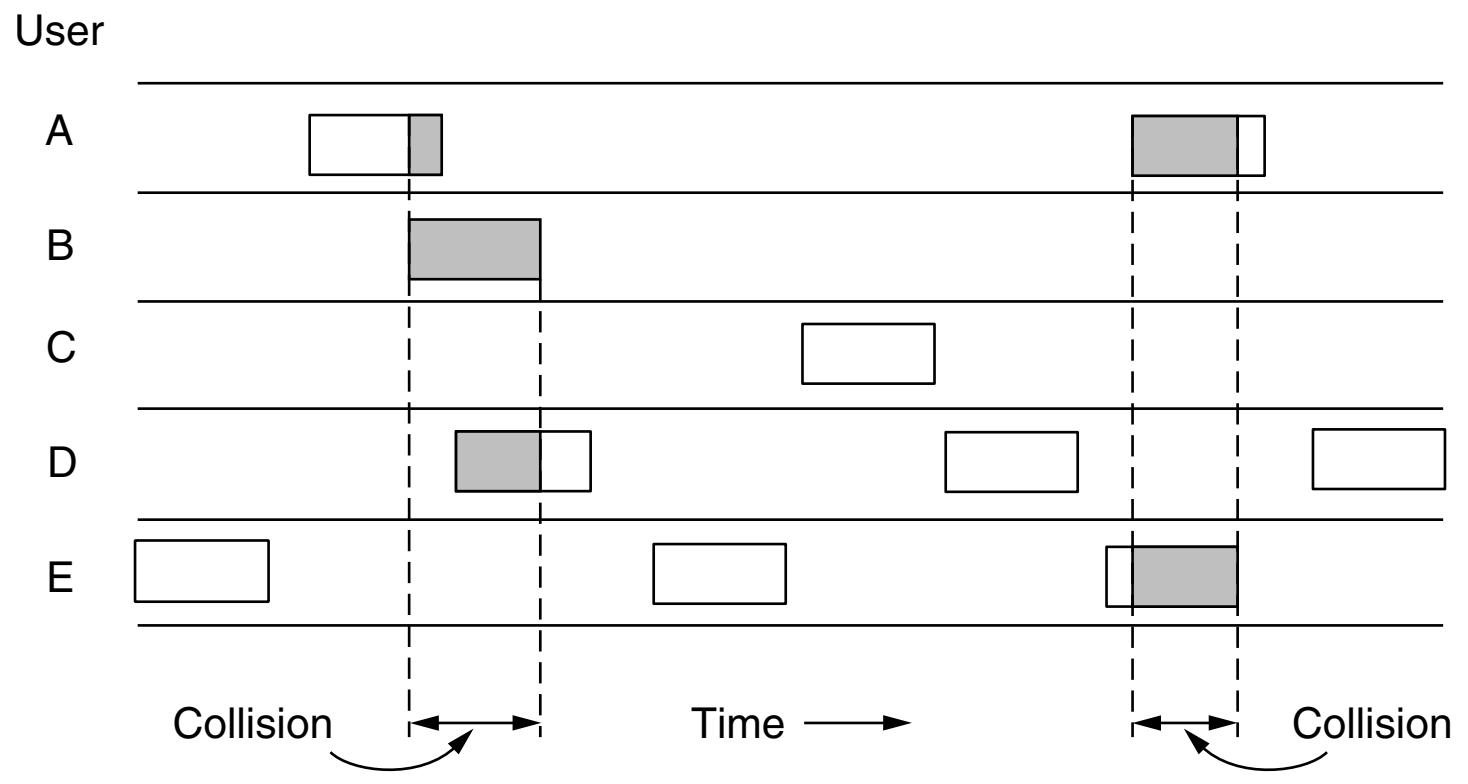
\includegraphics[scale=0.26]{image/aloha_conflict}
\end{center}
\caption{Các gói tin được truyền trong ALOHA \cite{6}}
\label{aloha_conflict}
\end{figure}
\begin{figure}[h]
\begin{center}
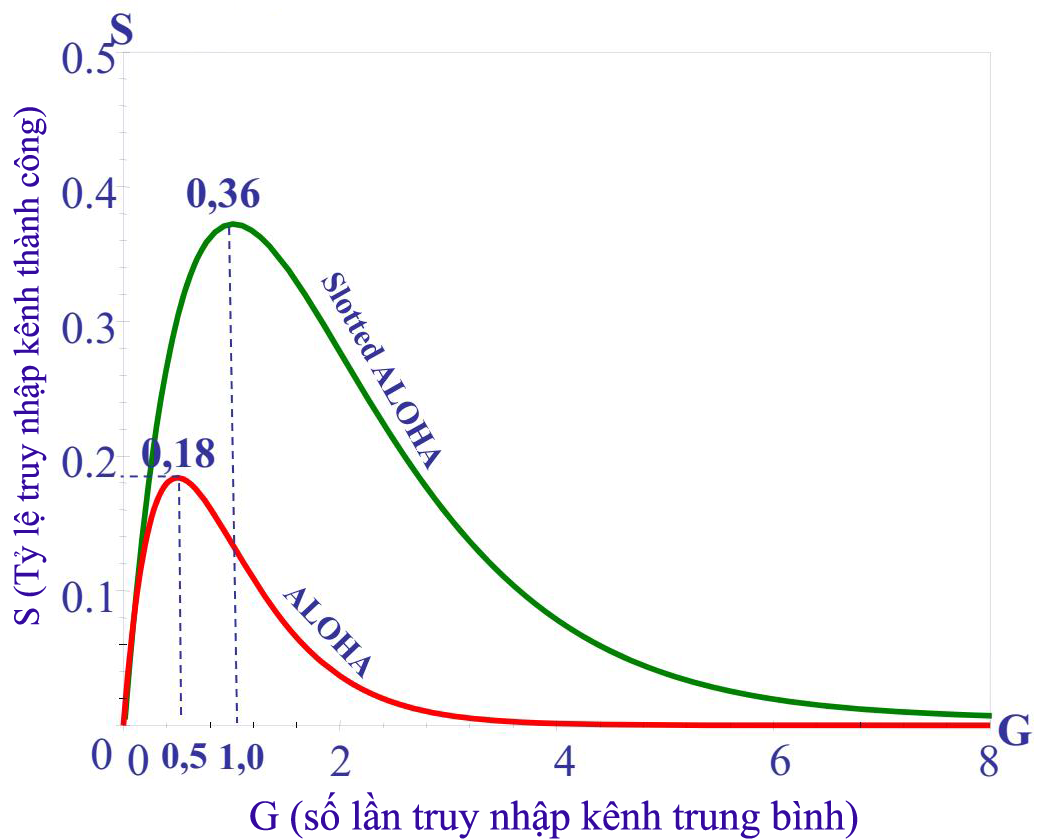
\includegraphics[scale=0.3]{image/efficiency_aloha}
\end{center}
\caption{Hiệu năng của hai giao thức ALOHA và Slotted ALOHA}
\label{efficiency_aloha}
\end{figure}
\par 
Do không có cách nào để kiểm soát xung đột trong ALOHA, nên hiệu năng của giao thức này khá thấp như thể hiện trong Hình \ref{efficiency_aloha}{}.
\subsubsection{Slotted Aloha}
Theo tài liệu \cite{6}, ngay sau ALOHA, vào năm 1972, Roberts đã công bố một phương pháp giúp tăng gấp đôi hiệu năng của hệ thống ALOHA. Đề xuất của ông là chia thời gian thành những khe thời gian rời rạc gọi là slot, bắt đầu của mỗi khe thời gian là lúc cho mỗi trạm tham gia kênh truyền. Phương pháp này yêu cầu các trạm phải thống nhất với nhau về khe thời gian. Một cách để có sự đồng bộ này là một trạm đặc biệt sẽ phát ra tín hiệu để thông báo bắt đầu khe thời gian. Hiệu năng của Slotted Aloha được mô tả trong Hình \ref{efficiency_aloha}{}.
\par 
Trong nắng năm 1970, sau khi được tạo ra, Slotted ALOHA được sử dụng trong các thí nghiêm và rồi nhanh chóng bị lãng quên cũng như ALOHA.
\subsection{Giao thức đa truy nhập dựa vào việc kiểm tra kênh truyền} 
Khi một trạm truyền bản tin, nó sẽ không biết các trạm khác đang làm gì, do vậy ở vùng giao của vùng phát sóng hai trạm sẽ xảy ra nhiều xung đột. Do đó, cần có một giao thức mà trạm có thể cảm nhận được kênh truyền. Có nhiều giao thức nghe kênh truyền đã được đưa ra, sau đây em xin trình bày một số phiên bản của giao thức đa truy nhập dựa vào việc cảm nhận kênh truyền CSMA (Carrier Sense Multiple Access).
\subsubsection{1-persistent CSMA}
1-persistent CSMA \cite{6} là giao thức đơn giản nhất trong các giao thức CSMA. Khi trạm có dữ liệu, đầu tiền nó sẽ cảm nhận kênh truyền xem các trạm khác có đang gửi tin không. Nếu kênh truyền rảnh, trạm sẽ gửi dữ liệu. Ngược lại, nếu kênh truyền bận, trạm sẽ chờ đến khi kênh truyền rảnh. Sau đó trạm sẽ truyền bản tin. Nếu va trạm xảy ra, trạm sẽ chờ một khoảng thời gian ngẫu nhiêu và bắt đầu gửi lại. Quá trình gửi tin của trạm sẽ được mô tả trong lưu đồ thuật toán Hình \ref{2CSMA}{}a. Tuy nhiên, trong trường hợp hai trạm cùng chờ chạm thức 3 thực hiện xong quá trình gửi tin, khi đó hai trạm sẽ cùng gửi tin, xung đột sẽ xảy ra. Giao thức 1-persistent CSMA có hiệu năng tốt hơn so với ALOHA do có quá trình kiểm tra kênh truyền.\\
\begin{figure}[h]
\centering
\subfigure[1-persistent CSMA.]
  {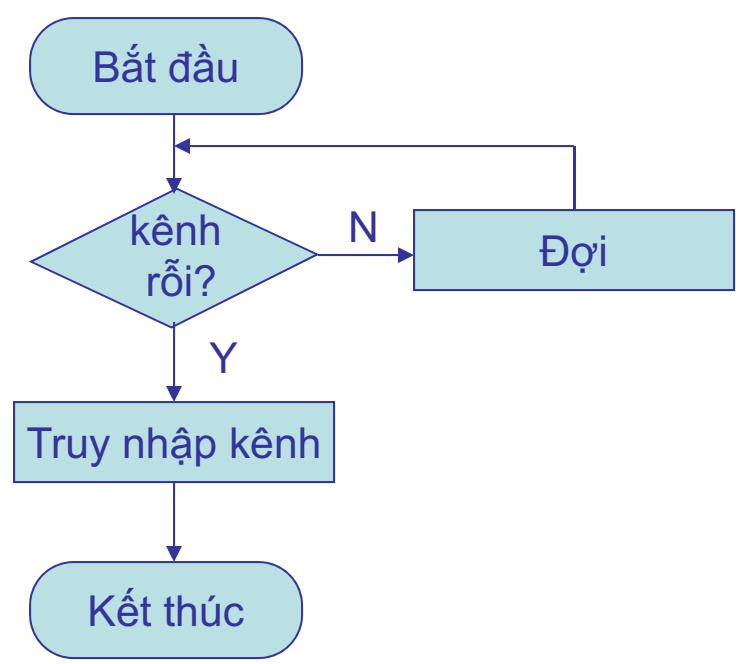
\includegraphics[width=.42\linewidth]{image/flowchart_1per}}
\hfill
\subfigure[non-persistent CSMA.]
  {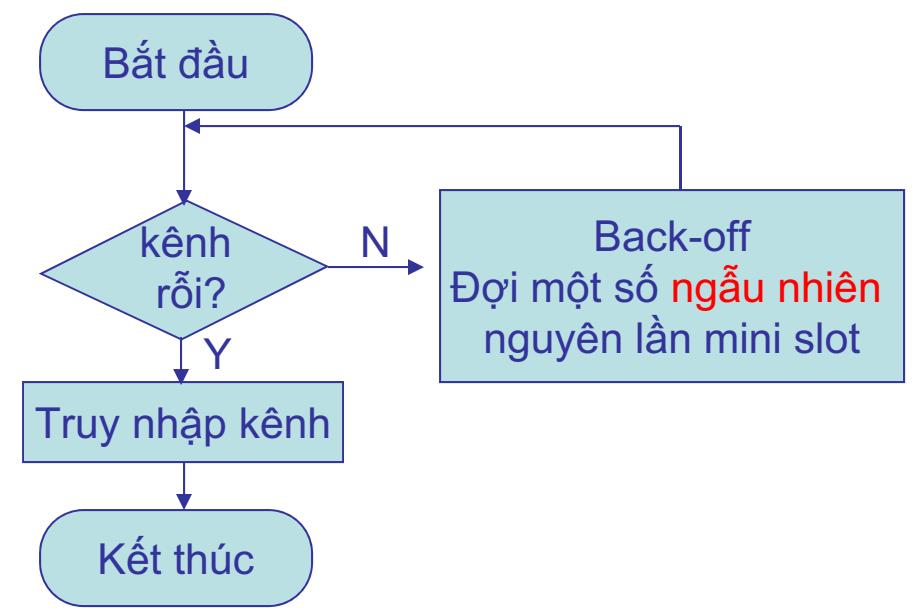
\includegraphics[width=.55\linewidth]{image/flowchart_nonper}}
\caption{Lưu đồ thuật toán của hai giao thức 1-persistent CSMA và non-persistent CSMA}
\label{2CSMA}
\end{figure} 
\subsubsection{Non-persistent CSMA}
Giao thức kiểm tra kênh truyền thức hai là nonpersistent CSMA. Theo tài liệu \cite{6}, cũng giống như 1-persistent CSMA, khi cảm nhận được kênh truyền rỗi, trạm sẽ gửi luôn bản tin. Tuy nhiên, khi kênh truyền bận, trạm sẽ không tiếp tục cảm nhận kênh truyền nữa mục đích để không cần ngay lập tức xác định thời điểm kết thúc của quá trình truyền tin trước. Thay vào đó, nó sẽ chờ một khoảng thời gian ngẫu nhiên rồi tiếp tục thuật toán. Hệ quả của quá trình này là sử dụng kênh truyền tốt hơn nhưng thời gian trễ dài hơn so với 1-persistent CSMA. Lưu đồ thuật toán Hình \ref{2CSMA}{}b mô tả giao thức nonpersistent CSMA.
\subsubsection{p-persistent CSMA}
Giao thức p-persistent CSMA \cite{6} khắc phục những nhược điểm của 1-persistent CSMA. Khi trạm sẵn sàng gửi dữ liệu, nó sẽ kiểm tra kênh truyền. Nếu kênh truyền rảnh, nó sẽ gửi dữ liệu với một xác xuất p hoặc đợi một mini slot (mini slot là khoảng thời gian nhỏ hơn rất nhiều so với thời gian truyền tối đa của tín hiệu) với xác xuất q = 1 - p sau đó kiểm tra lại kênh truyền. Khi kênh bận thì đợi kênh rỗi. Hình \ref{flowchart_pper} mô tả thuật toán của giao thức p-persistent CSMA. Giá trị xác suất p ảnh hưởng nhiều đến hiệu suất của kênh truyền.
\begin{figure}[h]
\begin{center}
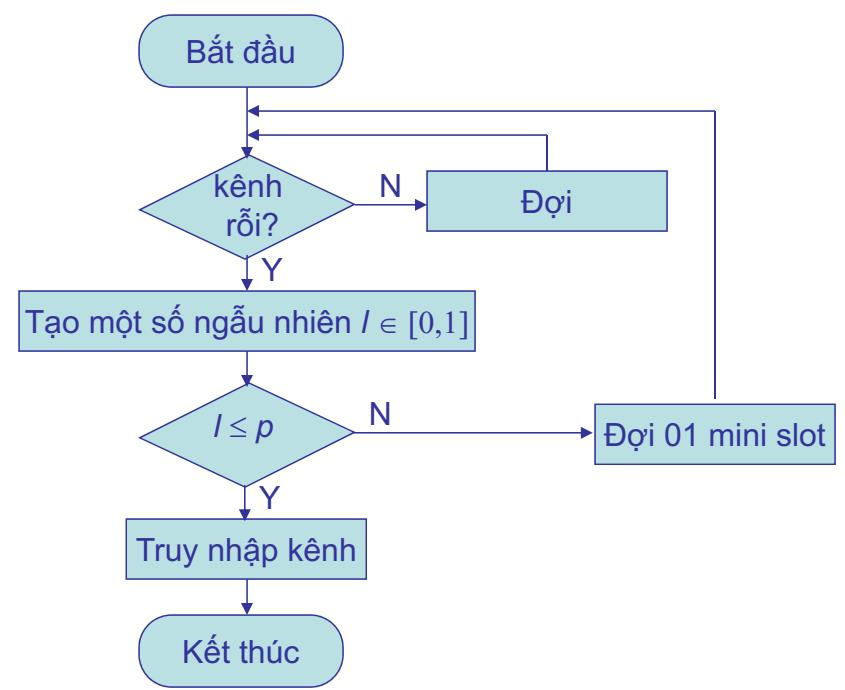
\includegraphics[scale=0.45]{image/flowchart_pper}
\end{center}
\caption{Lưu đồ thuật toán giao thức p-persistent CSMA.}
\label{flowchart_pper}
%\end{figure}//
%\begin{figure}
\begin{center}
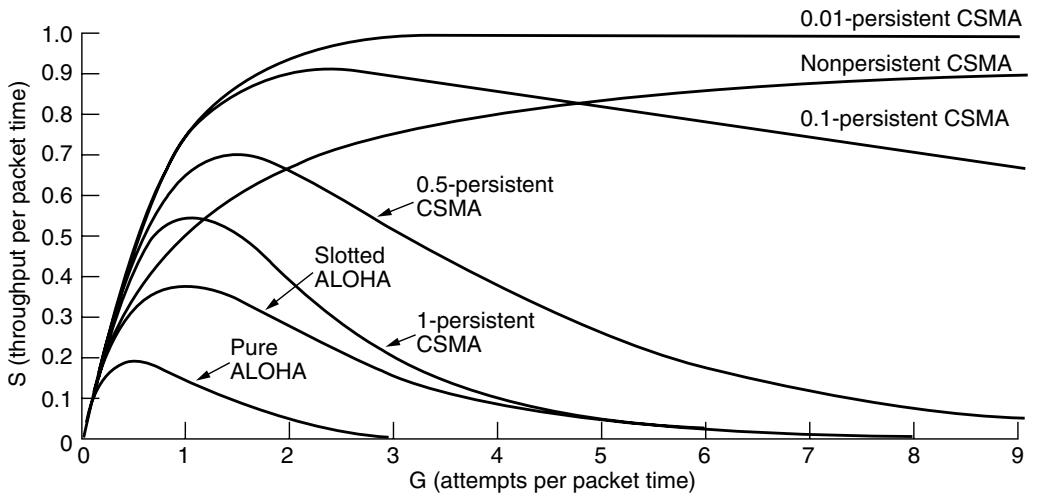
\includegraphics[scale=0.48]{image/compare}
\end{center}
\caption{So sánh hiệu năng sử dụng kênh truyền của các phương pháp truy nhập kênh truyền ngẫy nhiên \cite{6}{}.}
\label{compare}
\end{figure}
\par
Hình \ref{compare} so sánh hiệu suất của 3 giao thức 1-persistent CSMA, nonpersistent CSMA, p-persistent CSMA cũng như ALOHA và slotted ALOHA.
\subsubsection{CSMA/CA}
\begin{figure}[h]
\begin{center}
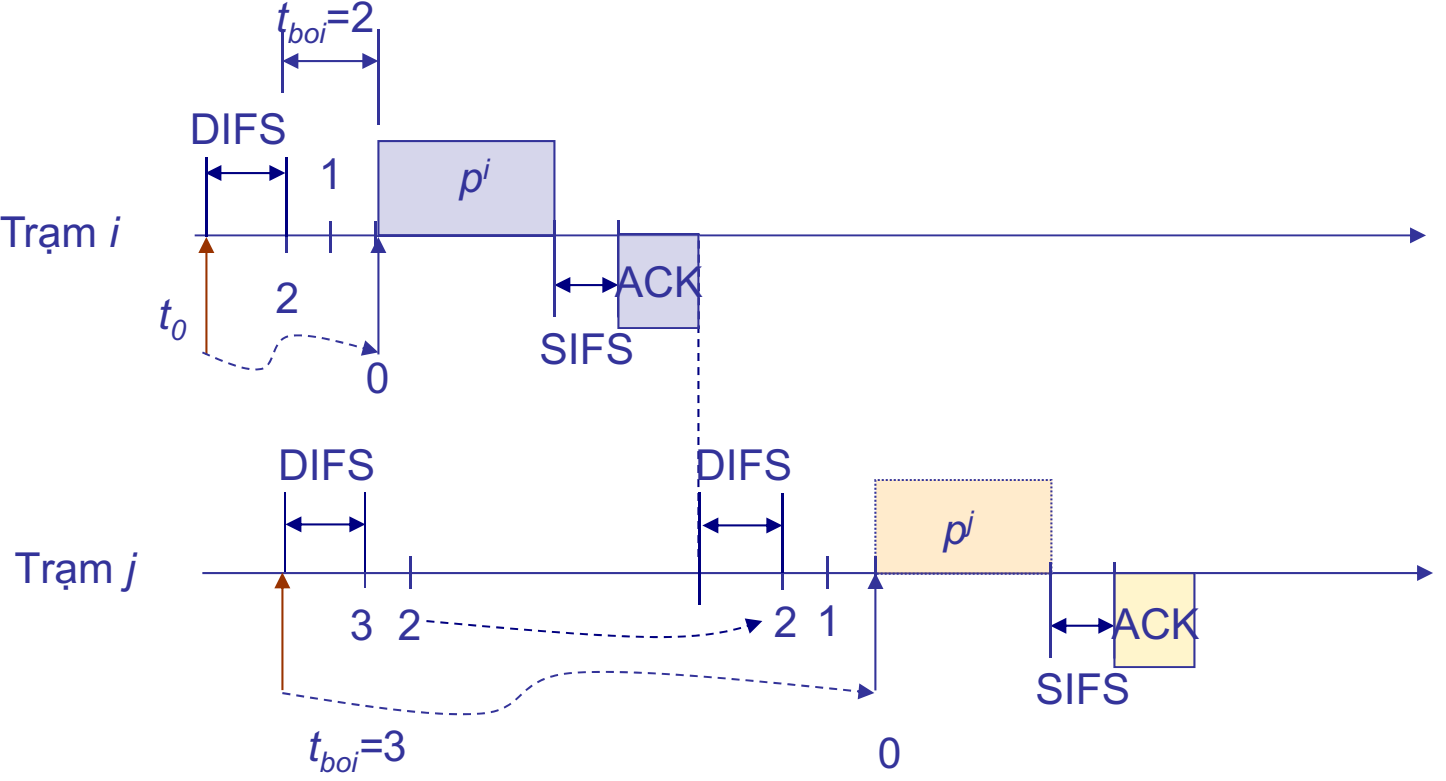
\includegraphics[scale=0.26]{image/CSMACA}
\end{center}
\caption{Quá trình truyền tin của 2 trạm sử dụng giao thức CSMA/CA}
\label{CSMACA}
\end{figure}
\noindent Do cơ chế kiểm tra trạng thái kênh truyền và cơ chế phát hiện va đập hoạt động không hiệu quả trong môi trường vô tuyền, nên cần có một giao thức CSMA được phát triển trong mạng vô tuyến đó là CSMA/CA (CSMA with Collision Avoidance). Cơ chế hoạt động của CSMA/CA (Hình \ref{CSMACA}{}):
\begin{itemize}
\item Trước khi truy nhập kênh truyền, kiểm tra trạng thái kênh truyền. Nếu xảy ra va đập, các trạm sẽ dừng truyền tin và gửi bản tin JAM SIGNAL để báo hiệu cho các trạm khác và back-off theo hàm mũ. Điều này có nghĩa, số lần truy nhập kênh truyền không thành công càng lớn thì thời gian back-off càng tăng,
\item Nếu kênh truyền bận: đợi đến khi kênh truyền rỗi,
\item Tiếp tục đợi thêm khoảng thời gian DIFS (DCF Inter-Frame Space) cho trước (DIFS = RTT),
\item Back-off một số mini slot $t_{BO}$ ngẫu nhiên,
\item Sau mỗi mini slot: $t_{BO} = t_{BO} - 1${},
\item  Nếu trong thời gian back-off kênh truyền lại bận thì trạm dừng đếm lùi và bảo toàn giá trị $t_{BO}$ tại thời điểm dừng,
\item Sau khi kênh truyền chuyển sang trạng thái rỗi một khoảng thời gian DIFS, trạm tiếp tục đếm lùi,
\item Nếu $t_{BO}$ = 0 thì truy nhập kênh và gửi gói.
\end{itemize}
\subsection{Giao thức đa truy nhập tránh va chạm MACA}
Ý tưởng cơ bản của giao thức MACA \cite{6} (Multiple Access with Collision Avoidance) (Karn, 1990) là sử dụng cơ chế tránh va đập. Quá trình truyền tin của trạm sử dụng giao thức MACA được mô tả trong Hình \ref{MACA}{}. Cơ chế tránh va đập gồm có các thành phần:
\begin{itemize}
\item Trước khi gửi: bên gửi sẽ quảng bá bản tin RTS (Ready-To-Send) cho các nút xung quanh biết là nó sắp sửa gửi bản tin,
\item Khi nhận được RTS: bên thu quảng bá bản tin CTS (Clear-To-Send) để cho bên nhận và các nút xung quanh nó biết nó sẵn sàng nhận bản tin,
\item Trong RTS và CTS mang theo bản tin NAV (Network Allocation Vector) chứa thời gian chiếm kênh truyền của bên phát,
\item Các trạm khác dừng việc truy nhập kênh truyền trong khoảng thời gian NAV.
\end{itemize}
\begin{figure}[h]
\begin{center}
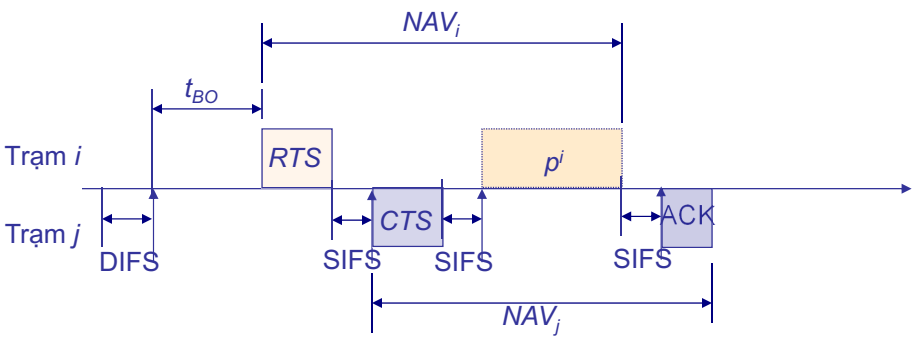
\includegraphics[scale=0.4]{image/MACA}
\end{center}
\caption{Quá trình truyền tin của hai trạm sử dụng giao thức MACA}
\label{MACA}
\end{figure}
Ở trên là một số giao thức đa truy nhập có thể áp dụng cho mạng không dây, mỗi giao thức có những ưu điểm và cũng có nhược điểm riêng. Đối với đề tài của mình, em xin lựa chọn việc xây dựng giao thức đa truy nhập của mình dựa trên giao thức ALOHA. Bởi vì, giao thức ALOHA đơn giản, dễ dàng triển khai. Ngoài ra, do dữ liệu cần truyền là nhỏ (dữ liệu lớn nhất trong một lần truyền là 255 byte), cùng với số lượng nút trong mạng ít nên rất phù hợp với việc ứng dụng giao thức ALOHA.
\section{Module LoRa Ai Thinker SX1278 Ra-02}
Ai Thinker là một hãng chuyên về lĩnh vực thiết kế và sản xuất module truyền thông không dây (WiFi, LoRa, GPRS,…) của Trung Quốc.
\par 
Module truyền thông LoRa SX1278 Ra-02 là một trong số những module sử dụng công nghệ LoRa có giá thành rẻ, sử dụng IC truyền thông LoRa SX1278 của Semtech. Hình ảnh module SX1278 cùng với sơ đồ chân và sơ đồ khối được thể hiện trong Hình \ref{SX1278}.
\begin{figure}[t]
	\centering
	\subfigure[Hình ảnh thực tế Module LoRa Ai Thinker SX1278 Ra-02 \cite{*}]
	{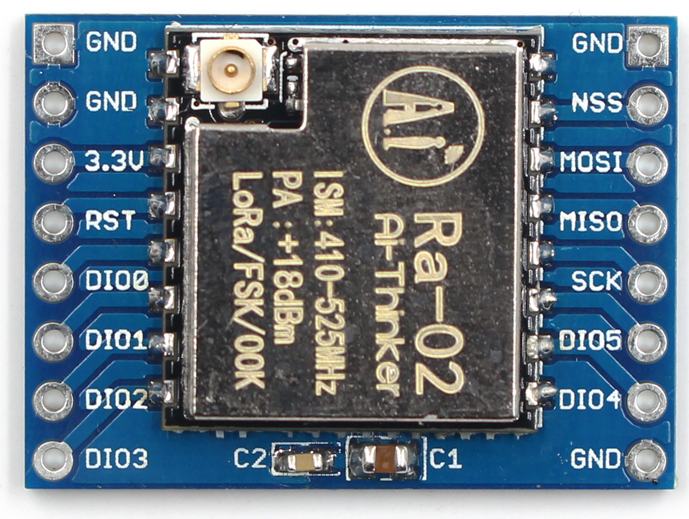
\includegraphics[width=0.45\linewidth]{image/hinh2_7}}
	\subfigure[Sơ đồ chân IC SX1278 \cite{8}]
	{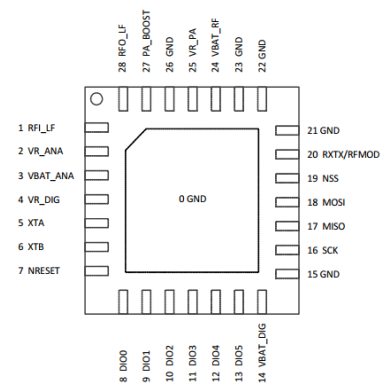
\includegraphics[width=0.46\linewidth]{image/hinh2_9}}\\
	\subfigure[Sơ đồ khối IC SX1278 \cite{8}]
	{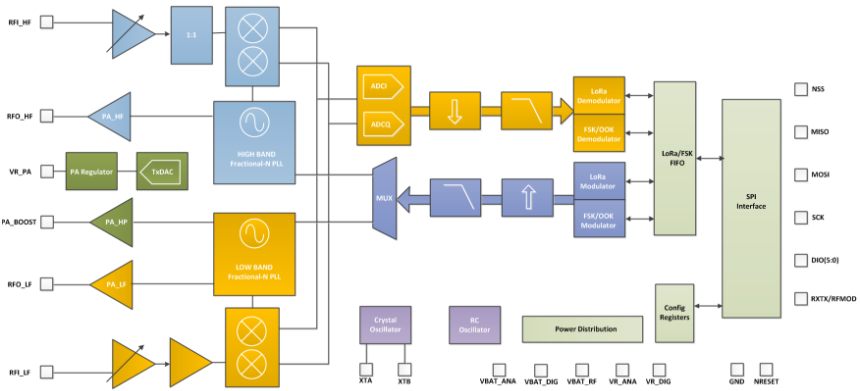
\includegraphics[scale=0.5]{image/hinh2_8}}%
\caption{Module LoRa Ai Thinker SX1278 Ra-02}
\label{SX1278}
\end{figure}
\par 
Thông số của module LoRa Ai Thinker SX1278 Ra-02 \cite{7} gồm có:
\begin{itemize}
\item Kích thước: 17 x 16 mm,
\item Hỗ trợ chuẩn giao tiếp SPI,
\item Hoạt động trên dải tần: 410 – 525 MHz,
\item Hỗ trợ công nghệ điều chế FSK, GFSK, GMSK và LoRa,
\item Điện áp hoạt động: 2.5 – 3.7,
\item Dòng điện tiêu thụ (Bảng \ref{bang2_1}),
\item Công suất phát: 18 $\pm$ 1 dBm,
\item Nhiệt độ hoạt động: -30 - 85 $^{\circ}$C .
\end{itemize}
\begin{table}[h]
    \centering
    \caption{Dòng điện tiêu thụ của module LoRa Ai Thinker SX1278~Ra-02 \cite{7}}
    \begin{tabular}{|c|c|c|c|}
     	\hline
     	Tần số & RX & TX & Standby \\
     	\hline
     	433 MHz & 93 mA & 12,15 mA & 1,6 mA \\
     	\hline
     	470 MHz & 97 mA & 12,15 mA & 1,5 mA \\
     	\hline
    \end{tabular}
    \label{bang2_1}
\end{table}
Theo datasheet của IC SX1278 do Semtech công bố \cite{8}, IC SX1278 là một trong những chip thu phát sóng điện từ sử dụng công nghệ LoRa, cung cấp một vùng phủ sóng rộng, tiêu thụ ít năng lượng và khả năng chống nhiễu tốt.
\section{Vi điều khiển STM32F103}
Vi điều khiển STM32F103 là loại vi điều khiển 32 bit với lõi ARM Cortex-M3 trên kiến trúc RICS của hãng STMicroelectronics (ST). Vi điều khiển lõi được sử dụng rộng rãi trong các thiết bị điện tử - tự động bởi khả năng xử lý vượt trội, kích thước nhỏ, dễ dàng cho việc lập trình. Vi điều khiển lõi ARM Cortex-M3 dựa trên kiến trúc ARMv7-M được thiết kế để tối ưu hóa hiệu suất cho các ứng dụng vi xử lý, có nhiều ngoại vi, khả năng đa kết nối đa năng, tương thích với nhiều công cụ (tools) nạp của nhiều hãng khác nhau, cho phép lập trình và phát triển các ứng dụng một cách nhanh chóng. Vi điều khiển Cortex-M3 tiêu thụ ít điện năng và chi phí thấp, đồng thời cung cấp khả năng tính toán cao. Dưới đây là một số thông số hoạt động của vi điều khiển STM32F103 \cite{9}{}:
\begin{itemize}
\item Tần số cao nhất: 72MHz,
\item Dung lượng bộ nhớ flash: 256 KB,
\item Dung lượng RAM: 48 KB,
\item Dải điện áp 2,0 V – 3,6 V.
\end{itemize}
\begin{center}
    \begin{figure}[h]
    \begin{center}
     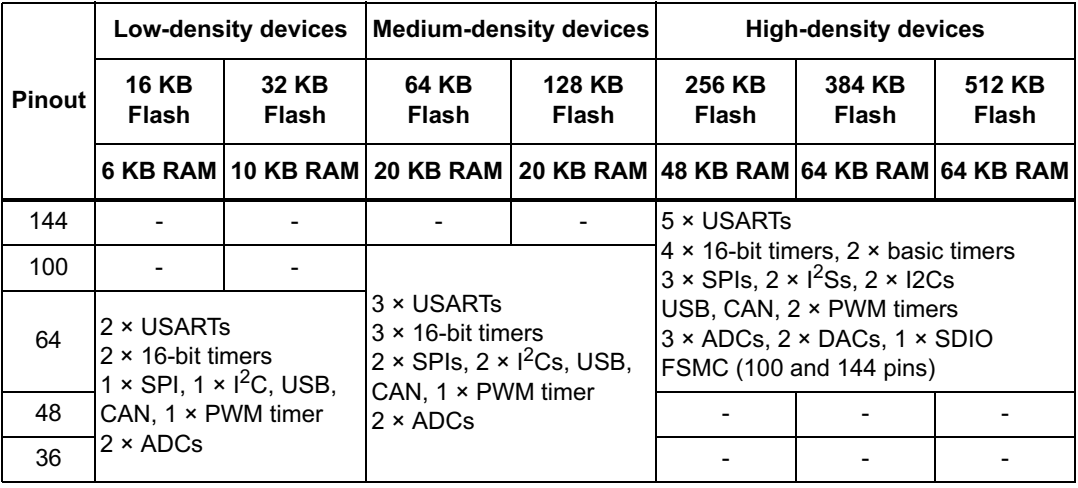
\includegraphics[scale=0.3]{image/bang2_2}
    \end{center}
    \caption{Thông số họ vi điều khiển STM32F103xxx \cite{9}}
    \label{refhinh2_9}
    \end{figure}
\end{center}
\par 
Bên cạnh đó, vi điều khiển STM32F103 còn hỗ trợ các tính năng sau \cite{9}:
\begin{itemize}
\item Bộ chuyển đổ ADC 12-bit,
\item Tích hợp Timer 16-bit với hai bộ điều khiển PWM,
\item Đầy đủ các kết nối thông dụng: I2C, SPI, I2S, CAN, USART,
\item Hỗ trợ các loại ngoại vi như SDIO, USB,
\item Hỗ trợ giao tiếp với ngoại vi thông qua các kênh DMA,
\item Nạp chương trình thông qua 2 phương thức SWD và Bootloader,
\item Tích hợp cảm biến nhiệt ngay trong CPU với độ phân giải 1 $^{\circ}$C.
\end{itemize} 
    \begin{figure}[h]
    \begin{center}
     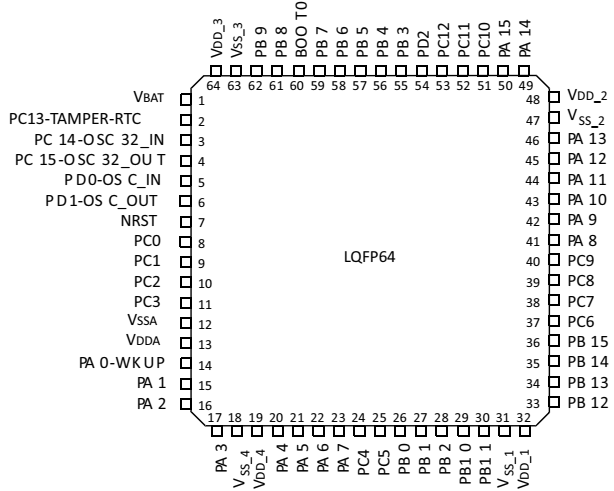
\includegraphics[scale=0.4]{image/hinh2_10}
    \end{center}
    \caption{Sơ đồ chân của dòng vi điều khiển STM32F103RCT6 64 chân \cite{9}}
    \label{refhinh2_10}
    \end{figure}
\section{Thiết bị giám sát các tham số môi trường nước BKRES}
Thiết bị giám sát tham số môi trường nước BKRES là sản phẩm của đề tài cấp Sở “NGHIÊN CỨU MÔ HÌNH MẠNG CẢM BIẾN KHÔNG DÂY GIÁM SÁT MÔI TRƯỜNG NƯỚC PHỤC VỤ PHÁT TRIỂN NUÔI TÔM CHÂN TRẮNG TẠI QUẢNG NINH” do thầy giáo TS. Nguyễn Hữu Phát làm chủ nhiệm. Đây là hệ thống cảm biến tự động thu thập dữ liệu về môi trường nước nặm của hồ nuôi trồng thủy sản và cảnh báo kịp thời khi có dấu hiệu bất thường trong môi trường nước.
\par 
Hệ thống tích hợp nhiều loại cảm biến, có thể đo đồng thời nhiều thông số của nước cùng lúc, cảnh báo tại chỗ mỗi khi các thông số vượt ngưỡng an toàn, kết hợp với trung tâm dữ liệu tập hợp, phân tích và dự đoán khả năng có thể xảy ra.
\par 
Các chức năng chính của hệ thống BKRES gồm có:
\begin{itemize}
\item Hệ thống đo đạc được 7 thông số môi trường nước (với thông số chu kỳ thời gian cho trước) bao gồm:
	\begin{itemize}
	\item Bốn thông số được đo trực tiếp (sử dụng cảm biến) gồm có:
 		\begin{itemize}
		\item	Hàm lượng Oxy trong nước,
		\item   Độ pH,
		\item	Nhiệt độ,
		\item	Nồng độ muối.
		\end{itemize}
	\item Ba thông số nội suy (tính toán từ các thông số đã đo được qua cảm biến):
 		\begin{itemize}
		\item	Nồng độ $NH_3$,
		\item	Nồng độ $H_2S$,
		\item	Nồng độ $NO_2$.
 		\end{itemize}
 	\end{itemize}
\item Hiển thị tại chỗ các thông số đo được lên LCD,
\item Cảnh báo cho người dùng khi các thông số vượt quá ngưỡng an toàn qua còi, đèn và qua SMS,
\item Lưu cấu hình vào bộ nhớ Flash để có thể phục hồi cấu hình khi bị mất điện,
\item Lưu lại nhật ký hệ thống vào thẻ nhớ (Có tùy chọn Bật/Tắt),
\item Mã hóa rồi gửi dữ liệu về máy chủ thông qua mạng di động,
\item Có khả năng điều chỉnh các thông số hệ thống từ xa qua máy chủ hoặc SMS (có mật khẩu),
\item Chu kỳ lấy dữ liệu, gửi dữ liệu về máy chủ, chu kỳ lưu giữ vào thẻ nhớ,
\item Cập nhật giá trị ngưỡng trên và dưới của thông số (Cho phép tự động cập nhật từ máy chủ),
\item Truy vấn thông tin hệ thống gồm các thông số cấu hình và tình trạng hệ thống,
\item Cập nhật và bảo trì hệ thống.
\end{itemize}
\par 
Yêu cầu khoa học cần đạt:
	\begin{itemize}
	\item Module phần cứng hoạt động ổn định trong môi trường khắc nghiệt, dễ dàng mở rộng, nâng cấp khi cần,
	\item Xử lý các dữ liệu từ cảm biến với tốc độ nhanh, tiêu tốn ít tài nguyên hệ thống nhất,
	\item Đảm bảo các phép tính toán có sai số ít nhất,
	\item Đảm bảo truyền thông tin cậy,
	\item Kích thước nhỏ gọn, tiêu thụ năng lượng thấp.
	\end{itemize}
\begin{figure}[h]
    \begin{center}
     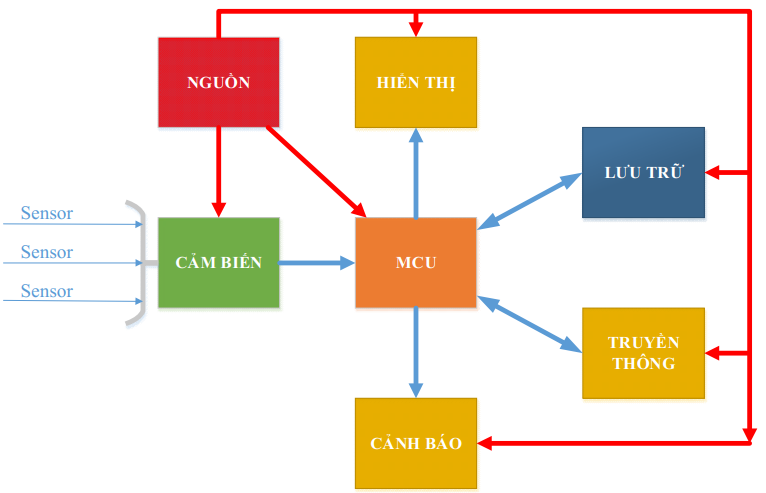
\includegraphics[scale=0.5]{image/hinh2_12}
    \end{center}
    \caption{Sơ đồ khối một thiết bị BKRES (client)}
    \label{refhinh2_12}
    \end{figure}
\par 
Máy chủ và thiết bị trao đổi dữ liệu qua việc trao đổi bản tin trên hạ tầng mạng GSM sử dụng giao thức TCP/IP nhằm đảm bảo dữ liệu truyền tải được chính xác và đầy đủ. Để máy chủ có thể nhận diện và giải mã dữ liệu được gửi đến thì phần dấu hiệu nhận diện bản tin và giá trị chỉ định kích thước bản tin cần được giữ nguyên không được mã hóa. Phần dữ liệu mã hóa chỉ bao gồm nội dung bản tin. Do đó, cấu trúc bản tin (Bảng 2.3) được xây dựng gồm có:
\begin{itemize}
\item HEADER: phần đầu bản tin và kích thước của toàn bộ bản tin,
\item Phần nội dung bản tin (phần được mã hóa) bao gồm:
  	\begin{itemize}
  	\item	Thông tin về ClientID,
  	\item	Loại bản tin (CommandID),
  	\item	Thông tin về thời gian (Timestamp),
  	\item 	Dữ liệu bản tin (Payload).
	\end{itemize}   
\item END: nhận diện kết thúc bản tin.
\end{itemize}
Nội dung bản tin xác thực gồm:
\begin{itemize}
\item Thông tin về phiên bản hệ thống,
\item Mã CODE (một thành phần tạo khóa AES),
\item Mã B (một thành phần tạo khóa AES),
\item Checksum.
\end{itemize}
Nội dung bản tin dữ liệu gồm:
\begin{itemize}
\item Thông tin về dữ liệu cảm biến: pH, Oxy, Salt, Temp, NH3, H2S,
\item Checksum.
\end{itemize} 
\begin{figure}[h]
    \begin{center}
     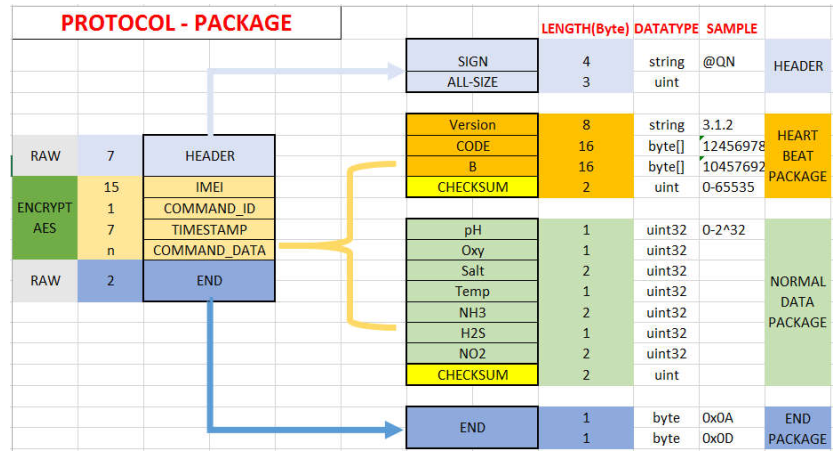
\includegraphics[scale=0.5]{image/hinh2_13}
    \end{center}
    \caption{Cấu trúc bản tin gửi dữ liệu trao đổi giữa máy chủ và client}
    \label{refhinh2_13}
\end{figure}
\par 
Hệ thống BKRES, sử dụng phương pháp truyền thông qua hệ thống GSM. Với việc sử dụng phương pháp này, mỗi thiết bị trong mạng cần phải có một module sim để truyền dữ liệu cho server, bên cạnh đó cần phải tốn chi phí hàng tháng để duy trì dịch vụ cho mỗi thiết bị. Phương pháp này có một số nhược điểm lớn là yêu cầu về cơ sở hạ tầng cao (cần có hệ thống GSM), khi hệ thống BKRES mở rộng (số lượng thiết bị lớn hơn) thì yêu cầu chi phí về việc duy trì hệ thống là lớn. Do đó, hệ thống BKRES hướng đến việc sử dụng công nghệ truyền thông LoRa để thu thập dữ liệu.
\section{Một số công cụ hỗ trợ khác}
\subsection{Phần mềm hỗ trợ cấu trình vi điều khiển}
Để cấu hình chức năng phần cứng cho các dòng vi điều khiển, ST đưa ra bộ công cụ STM32CubeMX \cite{10}. Phần mềm này hỗ trợ cấu hình các chức năng cho một vi điều khiển, phục vụ cho một dự án mới một cách trực quan, nhanh chóng. Ngoài ra, STM32CubeMX tự động download các driver mới nhất của ST dành cho các dòng chip của mình. Vì vậy đảm bảo các API của hãng sẽ luôn được cập nhật. Công cụ này còn hỗ trợ tự động sinh project mới với tùy chọn các IDE thông dụng. Giao diện phần mềm và giao diện cấu hình cho từng ngoại vi được thể hiện trong Hình \ref{refhinh2_14} và Hình \ref{refhinh2_15}{}.\\
\begin{figure}[h]
    \begin{center}
     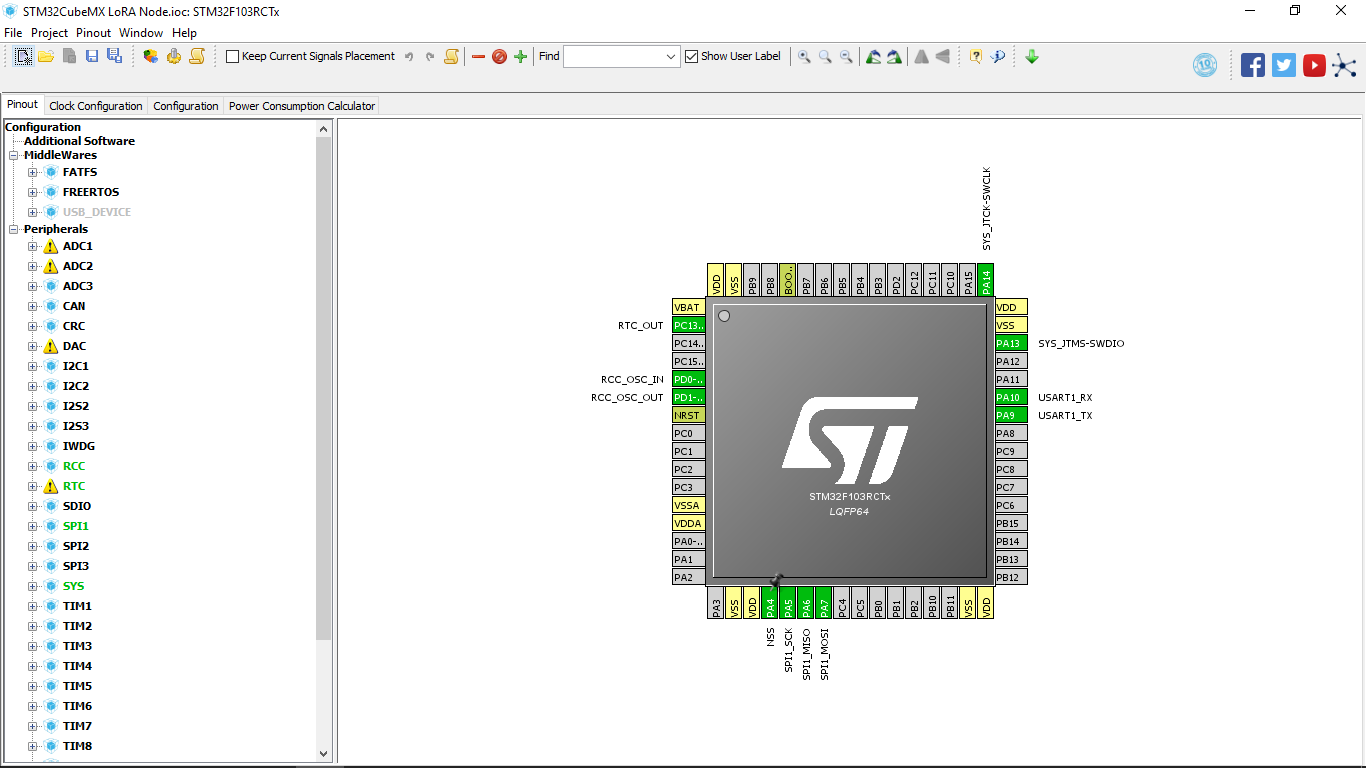
\includegraphics[scale=0.24]{image/hinh2_14}
    \end{center}
    \caption{Giao diện phần mềm STM32CubeMX hỗ trợ cấu hình}
    \label{refhinh2_14}
   \begin{center}
     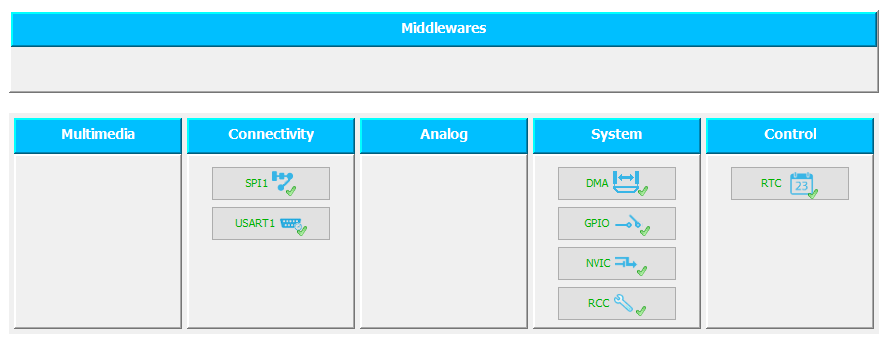
\includegraphics[scale=0.48]{image/hinh2_15}
    \end{center}
    \caption{Giao diện cấu hình chi tiết cho từng ngoại vi của STM32CubeMX}
    \label{refhinh2_15}
\end{figure}
\subsection{Phần mềm lập trình và biên dịch firmware Keil C}	
Keil C $\mu$Vision (Hình \ref{refhinh2_16}{}) là công cụ chuyên dụng hỗ trợ lập trình nhúng rất nổi tiếng. Keil C hỗ trợ hầu hết các loại chip vi xử lý trên thị trường và hỗ trợ 2 loại ngôn ngữ C/C++, Assembly. Nó được coi là IDE (môi trường phát triển) khá toàn diện, bao gồm khả năng biên dịch với trình biên dịch thương mại được tối ưu hóa, hỗ trợ nạp code và gỡ lỗi chuyên nghiệp.
\begin{figure}[h]
    \centering
     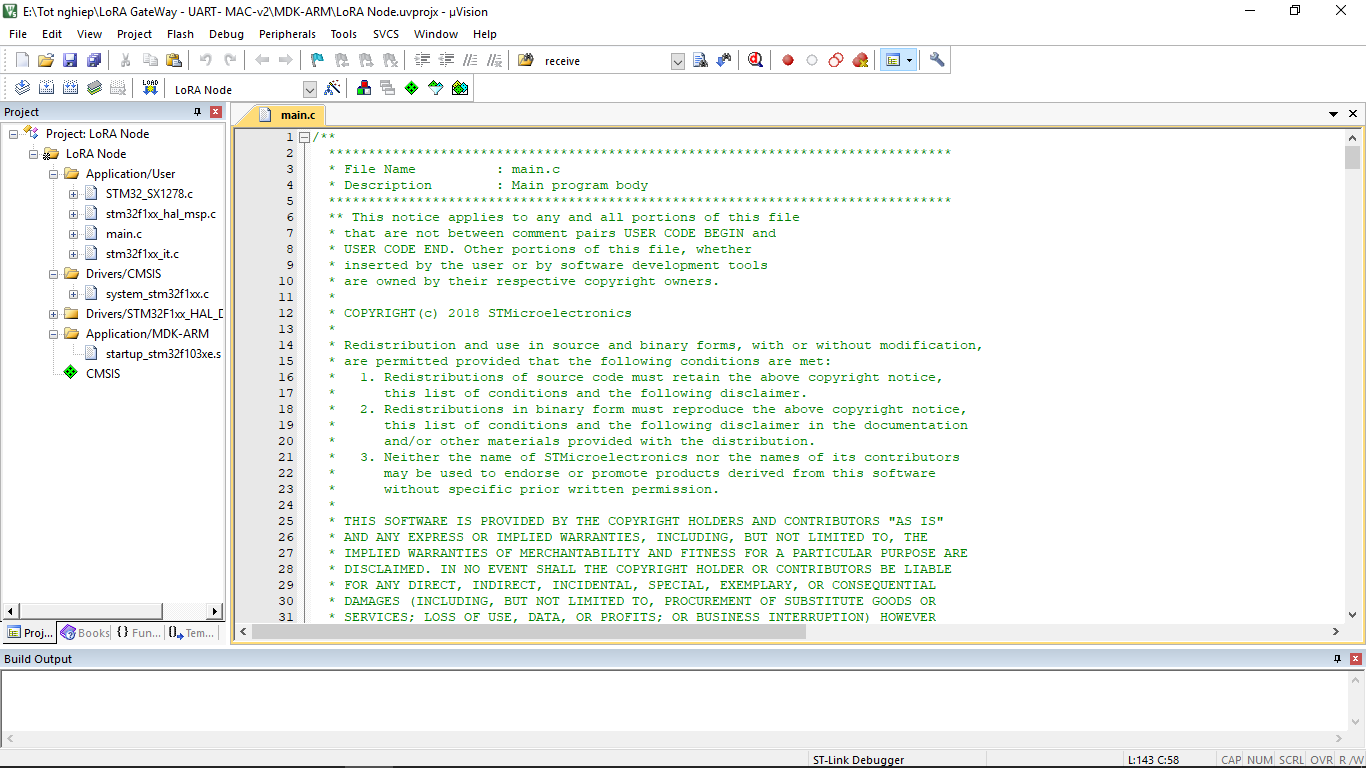
\includegraphics[scale=0.28]{image/hinh2_16}
    \caption{Giao diện phần mềm lập trình firmware Keil C $\mu$Vision}
    \label{refhinh2_16}
\end{figure}
\subsection{Phần mềm hỗ trợ giao tiếp UART Hercules} 
Trong quá trình lập trình, ngoài tính năng debug do phần mềm lập trình Keil C hỗ trợ, em còn sử dụng phần mềm Hercules (Hình \ref{refhinh2_17}{}) để hỗ trợ cho công việc kiểm tra và sửa lỗi. Hercules là một phần mềm hỗ trợ giao tiếp UART giúp hiển thị thông báo từ vi điều khiển lên máy tính, sử dụng đơn giản và thân thiện với người dùng. Sau khi kit kết nối với máy tính qua cổng COM, ta chỉ cần chọn đúng cổng COM được kết nối, chọn baud rate trùng với baud rate được cài đặt ở vi điều khiển, thế là có thể xem được thông báo từ vi điều khiển.\\
\begin{figure}[h]
\centering
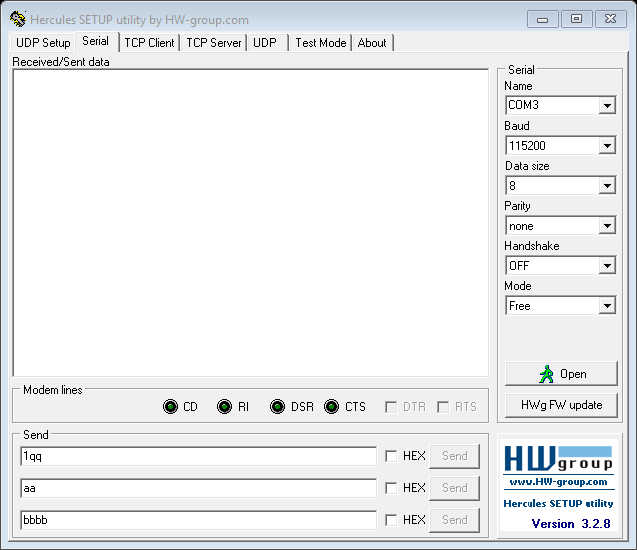
\includegraphics[scale=0.5]{image/hinh2_17}
\caption{Giao diện phần mềm HERCULES}
\label{refhinh2_17}
\end{figure}
\section{Kết luận}	
Từ những kiến thức em đã tìm hiểu và do những điểm phù hợp của ALOHA đối với hệ thống BKRES, em quyết định dựa trên giao thức ALOHA để xây dựng giao thức đa truy nhập và tích hợp giao thức đa truy nhập này vào thiết bị BKRES. Các bước tiến hành xây dựng giao thức sẽ được trình bày trong chương sau.





